\subsection{D(A) 上的幺半群结构}

命题 3. 设 \(\mathfrak{a}, \mathfrak{a}', \mathfrak{b}, \mathfrak{b}'\) 是 I(A) 中的元素。关系 \(\mathfrak{a} > \mathfrak{a}'\) 和 \(\mathfrak{b} > \mathfrak{b}'\) 蕴含 \(\mathfrak{ab} > \mathfrak{a}'\mathfrak{b}'\)。

我们可以把注意力限制在 \(\mathfrak{b} = \mathfrak{b}'\) 的情形。令 \(Ax\) 为包含 \(a'b\) 的分式主理想；对于每个非零元 \(y\)（\(\mathfrak{b}\) 中的），有 \(Ax \supset a'y\)，从而 \(Axy^{-1} \supset a'\)，于是 \(Axy^{-1} \supset a\) 且 \(Ax \supset ay\)。让 \(y\) 变化可见 \(Ax \supset ab\)，因此 \(ab > a'b\)。

由命题 3 可知，I(A) 上的乘法通过取商在 D(A) 上定义了一个合成律，该合成律显然满足结合律和交换律。我们采用加法记号，从而可以写成：

\[
\operatorname{div} (a b) = \operatorname{div} a + \operatorname{div} b,\tag{2}
\]

其中 a, b 属于 I(A)。显然 div(1) 是这个加法的单位元；将此元素记作 0。命题 3 进一步证明，D(A) 上的序结构与这个加法相容（《代数》第 VI 章，§ 1，第 1 节），更精确地说（第 1 节，命题 2 (ii)）：

\[
\begin{array}{r l} \inf (\operatorname{div} a + \operatorname{div} b, \operatorname{div} a + \operatorname{div} c) & = \inf (\operatorname{div} (a b), \operatorname{div} (a c)) = \operatorname{div} (a b + a c) \\ & = \operatorname{div} (a (b + c)) = \operatorname{div} a + \operatorname{div} (b + c) = \operatorname{div} a + \inf (\operatorname{div} b, \operatorname{div} c). \end{array}
\]

对于分式理想 \(a \neq 0\)，要使其在 D(A) 中满足 div \(a \geqslant 0\)，充要条件是 \(a \subset A\)（换句话说，a 是 A 的整理想）。

对于两个元素 \(x, y\)（属于 \(\mathbf{K}^*\)），关系 \(\operatorname{div}(x) = \operatorname{div}(y)\) 等价于 \(A x = A y\)；\(A\) 的主除子集合（带有由 \(D(A)\) 诱导的序关系和幺半群运算）是一个有序群，它典范同构于分式主理想的乘法群，后者按与包含关系相反的序排列（《代数》第 VI 章，§ 1，第 5 节）。记 \(S\) 为定义在两个元素 \(P, Q\)（\(D(A)\) 中）之间的关系：

\[
" \text { there   exists } x \in \mathbf {K} ^ {*} \text { such   that } \mathbf {P} = \mathbf {Q} + \operatorname{div} (x)"
\]

因而是等价关系，因为关系 \(P = Q + \text{div}(x)\) 等价于 \(Q = P + \text{div}(x^{-1})\)；如果 P 和 Q 模 S 同余，就称它们为 A 的等价除子。此外，关系 S 显然与幺半群 D(A) 的运算相容，因此后者通过取商在 D(A)/S 上定义了一个幺半群结构；这个幺半群称为 A 的除子类幺半群。

命题 4. 设 \(\mathfrak{a}\)、\(\mathfrak{b}\) 是 \(\mathbf{A}\) 的两个除性分式理想。以下性质等价：

\begin{enumerate}
\def\labelenumi{(\alph{enumi})}
\item
  div a 和 div b 是等价除子；
\item
  存在 \(x \in \mathbf{K}^*\)，使得 \(\mathfrak{b} = xa\)。
\end{enumerate}

若 \(\operatorname{div} \mathfrak{b} = \operatorname{div} \mathfrak{a} + \operatorname{div}(x)\) 对某个 \(x \in \mathbf{K}^*\) 成立，则 \(\operatorname{div} \mathfrak{b} = \operatorname{div}(xa)\)；由于 \(\mathfrak{b}\) 和 \(xa\) 都是除性的，故 \(\mathfrak{b} = xa\)，命题得证。

设 \(\mathfrak{a}\) 是一个可逆分式理想（第 II 章，§ 5，第 6 节）；则 \(\mathfrak{a} = \mathbf{A}\) : (A: \(\mathfrak{a}\) )（同上，命题 10），从而 \(\mathfrak{a}\) 是除性的（第 1 节，命题 1）。因此，可逆分式理想群 \(J(\mathbf{A})\) 可视为幺半群 \(D(\mathbf{A})\) 的一个子群，而 \(J(\mathbf{A})\) 在 \(D(\mathbf{A}) / S\) 中的典范像则与秩为 1 的投射 A-模的类群相同（第 II 章，§ 5，第 7 节，命题 12 的推论 2 及注 1）。

定理 1. 设 A 是整环。A 的除子幺半群 D(A) 为群的充要条件是 A 完全整闭。

假设 D(A) 是群。令 \(x \in K\)；假设 A{[}x{]} 包含于 K 的某个有限生成子 A-模中。我们已经看到（第 1 节），\(a = A[x]\) 是 I(A) 的元素。于是 \(xa \subset a\)，从而 \(\text{div}(x) + \text{div}a \geqslant \text{div}a\)。由于 D(A) 是有序群，我们得到 \(\text{div}(x) \geqslant 0\)，因而 \(x \in A\)。所以 A 完全整闭（第 V 章，§ 1，第 4 节，定义 5）。

反之，假设 A 完全整闭。设 a 是除性理想。我们将证明 \(\operatorname{div} a + \operatorname{div}(A: a) = 0\)，这将证明 \(\mathrm{D}(A)\) 是群。由于 \(a(A: a) \subset A\)，只需（第 1 节）验证：每个分式主理想 \(Ax^{-1}\) 若包含 \(a(A: a)\)，也包含 A。现在，对于 \(y \in K^{*}\)，关系 \(Ay \supset a\) 蕴含 \(y^{-1} \in A: a\)，从而 \(y^{-1}a \subset a(A: a) \subset Ax^{-1}\)，于是 \(xa \subset Ay\)。由于 a 是除性的，我们得到 \(xa \subset a\)，因此 \(x^{n}a \subset a\) 对所有 \(n \in N\) 都成立。存在元素 \(x_{0}, x_{1}\)（属于 \(K^{*}\)），使得 \(Ax_{0} \subset a \subset Ax_{1}\)；因此 \(x^{n}x_{0} \in Ax_{1}\)，从而 \(x^{n} \in Ax_{1}x_{0}^{-1}\)。由于 A 完全整闭，\(x \in A\)，即 \(Ax^{-1} \supset A\)，证明完毕。

注意，如果 A 完全整闭（甚至是诺特环），A 的除性理想未必可逆，换句话说，一般而言 \(J(A) \neq D(A)\)（习题 2 以及 § 3，第 2 节，命题 1）。

\pandocbounded{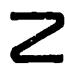
\includegraphics[keepaspectratio]{images/part003_63c67829.jpg}}

推论。设 A 是完全整闭整环，a 是 A 的除性分式理想。则对于 A 的每个非零分式理想 \(\mathfrak{b} \neq 0\)，有 \(\operatorname{div}(\mathfrak{a}: \mathfrak{b}) = \operatorname{div} \mathfrak{a} - \operatorname{div} \mathfrak{b}\)。

由第 1 节的公式 (1)：

\[
\operatorname{div} (a: b) = \operatorname{div} \left(\bigcap_ {\gamma \in b, \gamma \neq 0} \gamma ^ {- 1} a\right) = \sup _ {\gamma \in b, \gamma \neq 0} \operatorname{div} (\gamma ^ {- 1} a)
\]

这里用到了命题 2 以及分式理想 \(y^{-1}\mathfrak{a}\) 是除性的事实。不过，由于 \(\mathrm{D(A)}\) 是有序群（《代数》第 VI 章，§ 1，第 8 节）：

\[
\sup _ {\gamma \in b, \gamma \neq 0} \operatorname{div} (\gamma ^ {- 1} a) = \sup _ {\gamma \in b, \gamma \neq 0} (\operatorname{div} a - \operatorname{div} (\gamma)) = \operatorname{div} a - \inf _ {\gamma \in b, \gamma \neq 0} \operatorname{div} (\gamma) = \operatorname{div} a - \operatorname{div} b.
\]

